Voici une présentation de l'interface et ses fonctionnalités.

\subsection{Interface}
Voici comment se présente notre interface : 
\begin{figure}[!h]
    \centering
    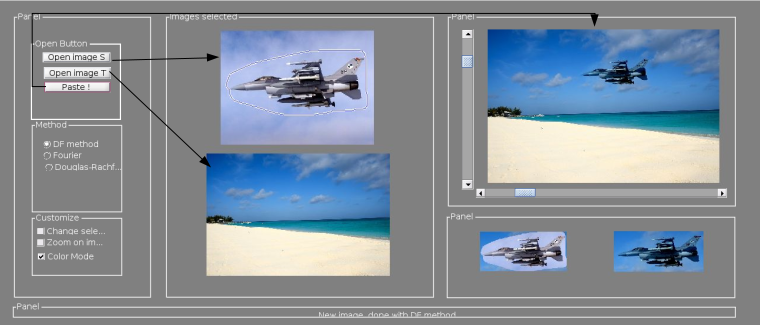
\includegraphics[scale = 0.2]{Images/interface.png}
    \caption{Interface 1.0}
\end{figure}{}
\subsubsection{Ouverture d'images}
Vous pouvez ouvrir n'importe quelle image en cliquant sur les boutons situés en haut à gauche de l'interface. E cliquant sur eux, une boite de dialogue vous proposera de choisir une image présente sur votre ordinateur. Une fois sélectionnée cette image sera affichée sur l'interface et vous pourrez travailler dessus. Image S correspond à l'image Source, c'est l'image que vous souhaitez coller. Et l'image T représente l'image Target, l'image d'arrière plan.\newline
Ici nous avons choisi d'ouvrir ces deux images. L'image à coller s'affichera dans le premier rectangle, celui le plus haut. Tandis que l'image d'arrière plan s'affichera en dessous de la première. 
\begin{figure}[!ht]
    \centering
    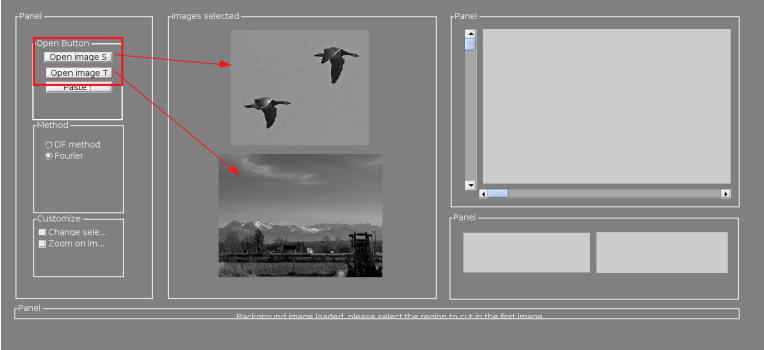
\includegraphics[scale = 0.3]{Images/images_ouvertes.png}
    \caption{Ouverture d'images}
\end{figure}{}
\subsubsection{Sélection}
Une fois vos deux images ouvertes, il vous faut sélectionner la partie de l'image S que vous souhaitez coller dans l'image T. Pour cela cliquez une première fois sur l'image S : celle du haut puis cliquez une seconde fois pour dessiner sur l'image, la partie que vous souhaitez extraire. 
\newline
Pour la seconde image, faites de même, cliquez une première fois sur l'image puis cliquez une seconde fois pour choisir l'endroit où vous souhaitez coller la partie sélectionnée plus tôt.  Voici ce que vous devriez obtenir. 
\begin{figure}[!ht]
    \centering
    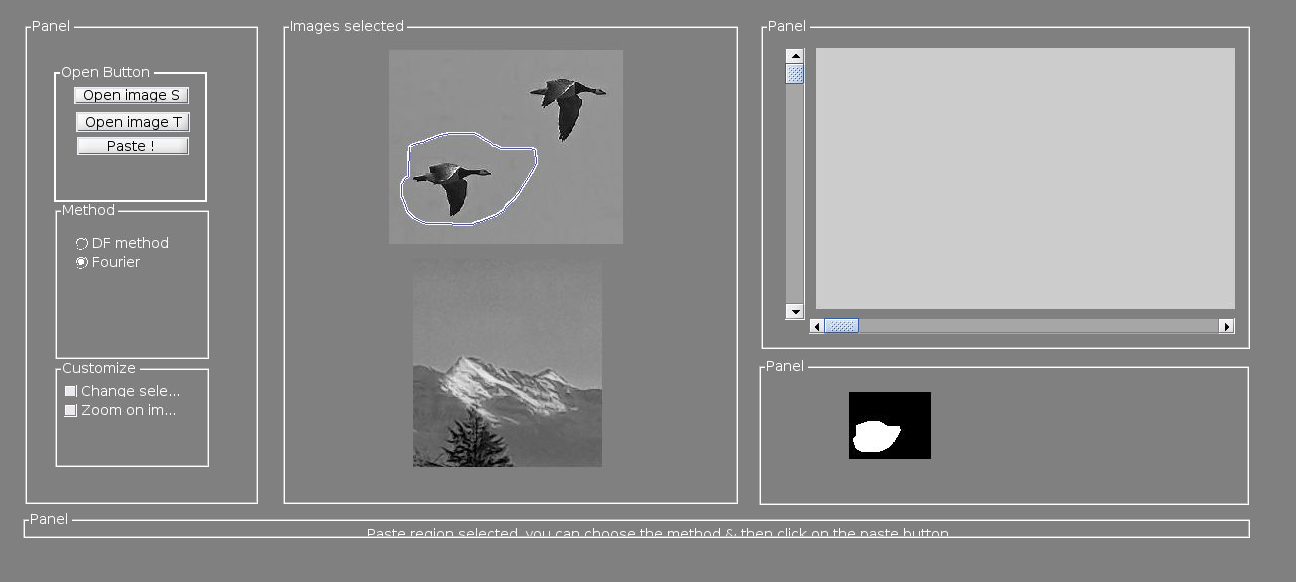
\includegraphics[scale = 0.2]{Images/selection.png}
    \caption{Sélection des parties}
\end{figure}{}
\subsubsection{Choix des méthodes}
Vous pouvez sélectionner la méthode avec laquelle vous voulez coller l'image S dans l'image T. Vous avez pour l'instant deux méthodes : 
\begin{itemize}
    \item Avec les différences finies
    \item Avec Fourier
\end{itemize}{}
\begin{figure}[!ht]
    \centering
    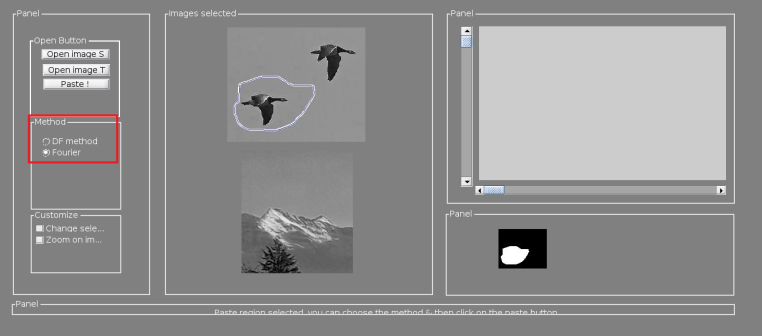
\includegraphics[scale = 0.3]{Images/method.png}
    \caption{Choisir une méthode}
\end{figure}{}

\subsubsection{Différences finies}
Une fois la méthode DF choisie, il vous suffit de cliquer sur le bouton "Paste!" pour afficher le résultat. Ce résultat s'affiche dans la partie droite de l'interface. 
\begin{figure}[!ht]
    \centering
    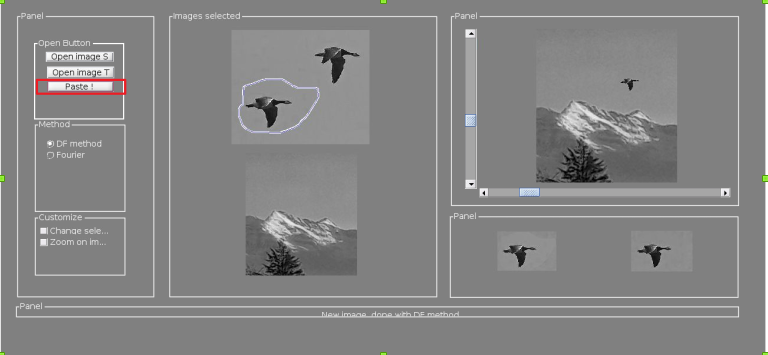
\includegraphics[scale = 0.3]{Images/DF.png}
    \caption{Différences finies}
\end{figure}{}
\newpage
\subsubsection{Fourier}
Pour afficher le résultat obtenus avec Fourier, il suffit de cocher la case Fourier
\begin{figure}[!h]
    \centering
    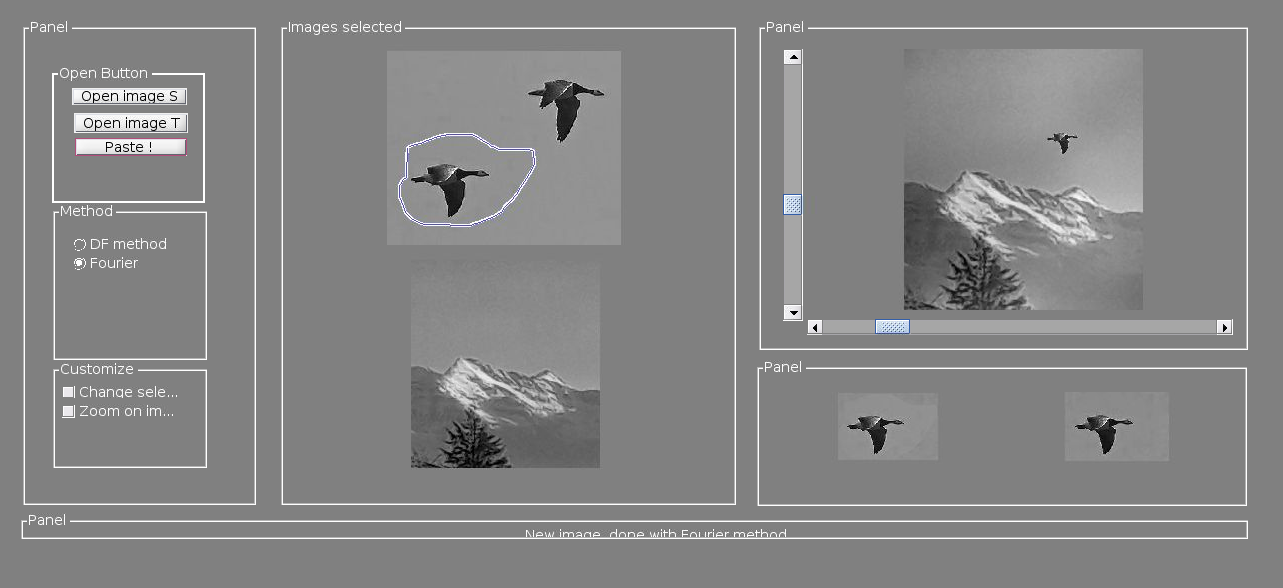
\includegraphics[scale = 0.2]{Images/fourier.png}
    \caption{Résultat obtenu avec la méthode de Fourier}
\end{figure}{}
Nous avons ajoutés des options comme l'option de zoom qui permet de zoomer sur une image pour voir de plus près le collage de l'image. 

\begin{figure}[!h]
    \centering
    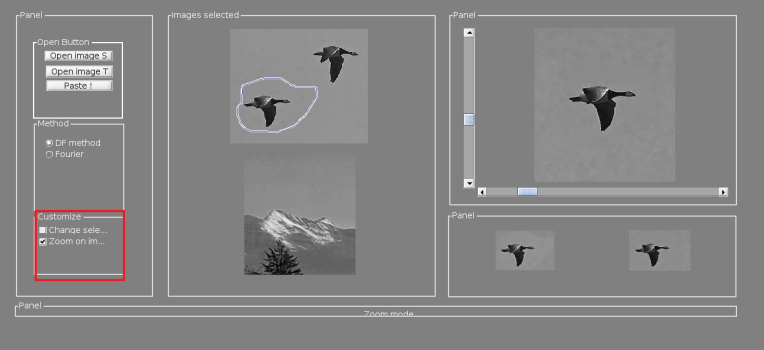
\includegraphics[scale = 0.3]{Images/zomm.png}
    \caption{Zoom}
\end{figure}{}
\subsubsection{Amélioration avec change selection}
\textbf{ATTENTION CETTE FONCTIONNALITE NE FONCTIONNE POUR L'INSTANT QU'AVEC LA METHODE DES DIFFERENCES FINIES}
Nous avons aussi remarquer un problème en effectuant différents tests sur les images : 
\begin{figure}[!ht]
    \centering
    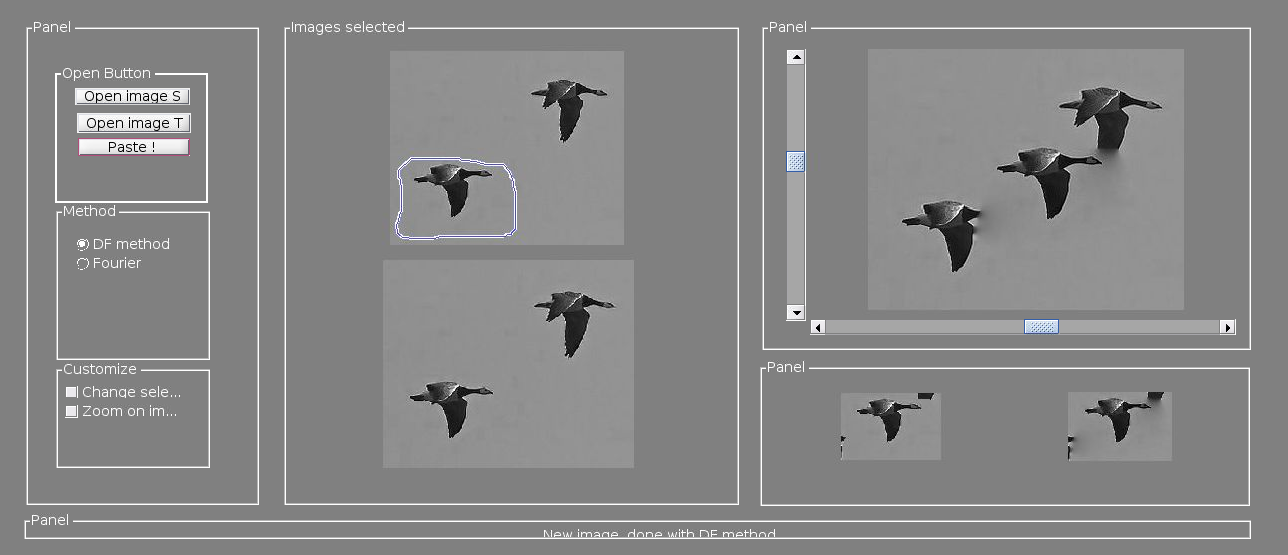
\includegraphics[scale = 0.15]{Images/pb.png}
    \caption{Problème de collage}
\end{figure}{}
Ainsi nous avons ajouté, l'option Change sélection qui re-dimensionne automatique la sélection afin de résoudre ce pb. 
\begin{figure}[!ht]
    \centering
    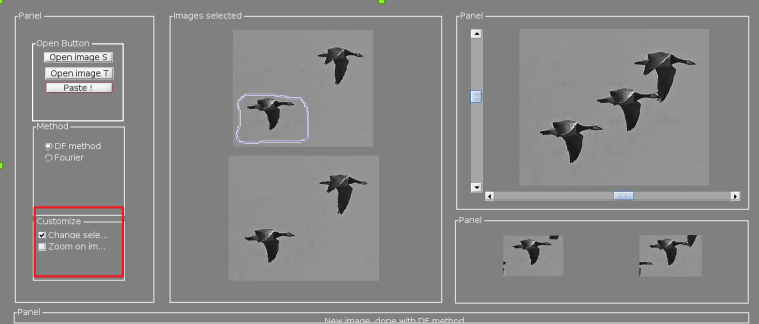
\includegraphics[scale = 0.3]{Images/solve.png}
    \caption{Résolution du problème}
\end{figure}{}

\subsubsection{Sliders}
Vous pouvez bouger les sliders présents à droite afin de déplacer la zone collée dans l'image de fond. La solution au problème est alors automatiquement recalculée en fonction de l'endroit où l'objet à collé. 
\begin{figure}[!h]
    \centering
    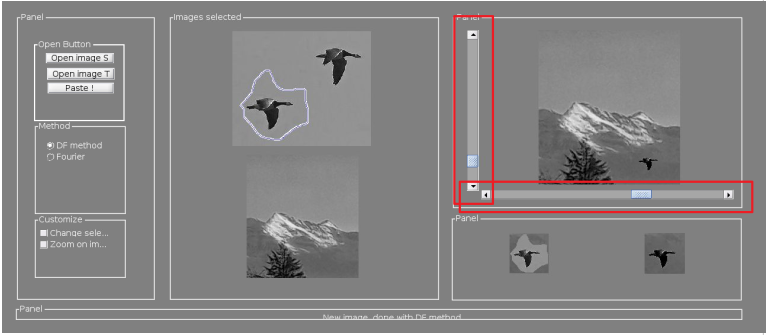
\includegraphics[scale = 0.2]{Images/move.png}
    \caption{Modifier l'endroit de collage}
\end{figure}

\subsection{Organisation du code}
Nous avons organisé le code sous forme de classes. Le projet contient 2 classes principales, la classe, Fourier et la classe DFinies

%%%%%%%%%%%%%%%%%%%%%%%%%%%%%%%%%%%%%%%%%%%%%%%%%%%
\begin{center}
\textbf{Classe Fourier}\\
\end{center}
\textbf{Propriétés}\\
\begin{itemize}
\item $grad_Tj$, $grad_Ti$ : permet de stocker le gradient de T, l'image d'arrière-plan\\
\item $grad_Sj$, $grad_Si$  : Permet de stocker le gradient de S, l'image à coller. \\
\end{itemize}
\textbf{Méthodes}
\begin{itemize}
\item compute\_grad : permet de calculer le gradient d'une image.
\item symmetry : Permet d'étendre l'image par symétrie, alors la taille de l'image est multipliée par 2. \\ 
solve : utilise la formule [], pour trouver la solution de l'équation de Poisson à l'aide de la méthode de Fourier. 
\item resize : permet de redimensionner l'image qui avait été symétrisée auparavant.
\end{itemize}
%%%%%%%%%%%%%%%%%%%%%%%%%%%%%%%%%%%%%%%%%%%%%%%%%%%%
\begin{center}
\textbf{Classe DFinies}\\
\end{center}
\textbf{Propriétés}\\
\begin{itemize}
\item $size$ : taille de la matrice.
\item matrix : permet de stocker la matrice du système.
\item vector : permet de stocker le vecteur b associé au système.
\item $i_vect$ : Permet de stocker les numéros de lignes de la matrice creuse A
\item $j_vect$ : Permet de stocker les numéros des colonnes de la matrice creuse A
\item $v_vect$ : Permet de stocker les coefficients de la matrice creuse A
\end{itemize}
\textbf{Méthodes}
\begin{itemize}
\item $add\_four$ : ajoute à la matrice creuse le coefficient -4, à la position i, j
\item $pix\_up\_is\_inside$ : ajoute le coefficient 1 à la matrice creuse, à la position
\item $pix\_down\_is\_inside$ : ajoute le coefficient 1 à la matrice creuse, à la position
\item $pix\_left\_is\_inside$ : ajoute le coefficient 1 à la matrice creuse, à la position
\item $pix\_right\_is\_inside$ : ajoute le coefficient 1 à la matrice creuse, à la position
\item $is\_inside$ : 
\item $find\_roi$ :  Trouve la région d'intérêt dans l'image
\item $find\_useless$ : Trouve les pixels, ne faisant pas partie de ma sélection
\item $create\_matrix$  : Crée la matrice A, pour résoudre le système.
\item $Laplacian$ :  Calcule le laplacien d'une image et met à jour le vecteur b.
\item solve :  Résout le système Ax=b et trouve l'image finale.
\end{itemize}

%%%%%%%%%%%%%%%%%%%%%%%%%%%%%%%%%%%%%%%%%%%%%%%%%%%%
\begin{center}
\textbf{Classe Mask}\\
\end{center}
\textbf{Propriétés}\\
\begin{itemize}
\item $associate\_im$
\item $associate\_roi$
\item $matrix$
\item $pos$
\item $pos\_to\_move$
\item $cut\_im$
\item $shift\_done$
\item $boundaries$
\end{itemize}
\textbf{Méthodes}
\begin{itemize}
\item $reinitialize\_mask$
\item $save\_mask\_settings$
\item $move\_roi$
\item $ivert\_mask$
\item $find\_boudaries$
\item $modify\_mask\_values$
\item $adjust\_size$
\item $change\_selection$
\end{itemize}
\begin{center}
\textbf{Fonction Copy/Paste}
\end{center}